\section{Aufbau}
    Im Folgenden wird der Aufbau des Algoritmus näher beschrieben. 
    Nach einem kurzem Überblick werden die einzelnen Subsysteme detailiert erklärt.
    \subsection{Grundlegende Struktur}
    % oberflächliche Beschreibung des systems
    Die Grundlegende Struktur lässt sich im wesentlichen durch das unten gegebene Baumdiagramm !!!FIGURE!!! beschreiben.
    
    \subsection{Aufbau im Detail - Mode}
        

    \subsection{Aufbau im Detail - Map}
    \begin{figure}
        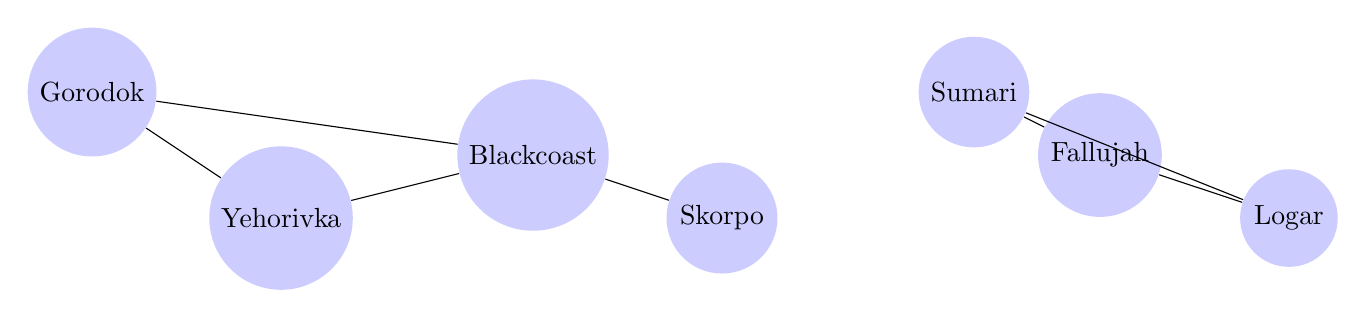
\begin{tikzpicture}
            [scale=.8,auto=left,every node/.style={circle,fill=blue!20}]
            \node (n1) at (1,10) {Gorodok};
            \node (n2) at (4,8)  {Yehorivka};
            \node (n3) at (8,9)  {Blackcoast};
            \node (n4) at (11,8) {Skorpo};
            \node (n5) at (15,10) {Sumari};
            \node (n6) at (20,8)  {Logar};
            \node (n7) at (17,9)  {Fallujah};
            \foreach \from/\to in {n1/n2,n1/n3,n2/n3,n3/n4,n5/n6,n5/n7,n6/n7}
            \draw (\from) -- (\to);  
        \end{tikzpicture}
    \caption{Cluster}
    \end{figure}

    \subsection{Aufbau im Detail - Layer}
    